\documentclass[12pt,a4paper]{report}

% ============================================
% PACKAGES
% ============================================
\usepackage[margin=1in]{geometry}           % Page margins
\usepackage{graphicx}                       % For including images
\usepackage{setspace}                       % Line spacing
\usepackage{titlesec}                       % Chapter/section formatting
\usepackage{tocloft}                        % Table of contents formatting
\usepackage{mathptmx}                       % Times-like font
\usepackage[utf8]{inputenc}                 % UTF-8 encoding
\usepackage{hyperref}                       % Clickable links in TOC
\usepackage{caption}                        % Figure captions
\usepackage{enumitem}                       % Better list formatting

% ============================================
% FORMATTING SETTINGS
% ============================================
\onehalfspacing                             % 1.5 line spacing

% Chapter formatting
\titleformat{\chapter}[display]
  {\normalfont\huge\bfseries}{\chaptertitlename\ \thechapter}{20pt}{\Huge}
\titlespacing*{\chapter}{0pt}{0pt}{40pt}

% Section formatting
\titleformat{\section}
  {\normalfont\Large\bfseries}{\thesection}{1em}{}
\titleformat{\subsection}
  {\normalfont\large\bfseries}{\thesubsection}{1em}{}

% Hyperref settings
\hypersetup{
    colorlinks=true,
    linkcolor=black,
    urlcolor=blue,
    citecolor=black
}

% ============================================
% DOCUMENT BEGINS
% ============================================
\begin{document}

% ============================================
% FRONT MATTER (Roman numerals)
% ============================================
\pagenumbering{roman}

% --------------------------------------------
% TITLE PAGE
% --------------------------------------------
\begin{titlepage}
    \centering

    \vspace*{1cm}

    % NITM Logo placeholder
    % TODO: Replace with actual logo
    % 
\includegraphics[width=3cm]{nitm_logo.png}
    {\Large [NITM LOGO HERE]}

    \vspace{1.5cm}

    {\LARGE\bfseries INTERNSHIP REPORT}

    \vspace{1cm}

    {\Large On}

    \vspace{0.5cm}

    {\LARGE\bfseries EDGE AI HARDWARE AND SOFTWARE DEVELOPMENT}

    \vspace{1cm}

    {\Large At}

    \vspace{0.5cm}

    {\LARGE\bfseries PAMIR AI}

    \vspace{0.3cm}

    {\large Marina Blvd, San Francisco, CA, 94123-1284, United States}

    \vspace{1.5cm}

    {\large Submitted in partial fulfillment of the requirements}

    {\large for the award of the degree of}

    \vspace{0.5cm}

    {\Large\bfseries MASTER OF COMPUTER SCIENCE AND ENGINEERING}

    \vspace{1cm}

    {\large by}

    \vspace{0.5cm}

    {\Large\bfseries UTSAV BALAR}

    {\large Roll No: T24CS003}

    \vfill

    {\large\bfseries DEPARTMENT OF COMPUTER SCIENCE AND ENGINEERING}

    {\large\bfseries NATIONAL INSTITUTE OF TECHNOLOGY, MEGHALAYA}

    {\large BIJNI COMPLEX, LAITUMKHRAH, SHILLONG -- 793003}

    \vspace{0.5cm}

    {\large\bfseries 2025}

\end{titlepage}

% --------------------------------------------
% CERTIFICATE FROM THE COMPANY
% --------------------------------------------
\newpage
\chapter*{Certificate from the Company}
\addcontentsline{toc}{chapter}{Certificate from the Company}

\vspace{1cm}

This is to certify that \textbf{Utsav Balar}, Roll No. \textbf{T24CS003}, student of Master of Computer Science and Engineering at National Institute of Technology, Meghalaya, has been working as a full-time intern at \textbf{Pamir AI} since \textbf{31st May 2025} and is currently continuing with the company.

\vspace{0.5cm}

During this ongoing internship, he has worked on various projects related to Linux kernel development, BSP engineering, and edge AI hardware integration. His work includes developing custom kernel drivers, creating software development kits, and implementing system services for our Distiller product line.

\vspace{0.5cm}

He has shown excellent technical skills, dedication, and commitment throughout this long-term internship. His contributions have been valuable to our product development efforts.

\vspace{0.5cm}

We wish him all the best for his future endeavors.

\vspace{2cm}

\noindent
\textbf{Tianqi Ye} \\
Co-founder and CTO \\
Pamir AI

\vspace{1.5cm}

\noindent
\textbf{Signature:} \underline{\hspace{6cm}}

\vspace{0.5cm}

\noindent
\textbf{Date:} \underline{\hspace{4cm}} \hspace{1cm} \textbf{Place:} \underline{\hspace{4cm}}

% --------------------------------------------
% CERTIFICATE FROM THE INSTITUTE
% --------------------------------------------
\newpage
\chapter*{Certificate from the Institute}
\addcontentsline{toc}{chapter}{Certificate from the Institute}

\vspace{1cm}

This is to certify that the internship report entitled \textbf{``Edge AI Hardware and Software Development''} submitted by \textbf{Utsav Balar}, Roll No. \textbf{T24CS003}, is a record of bonafide work carried out by him under my supervision and guidance in partial fulfillment of the requirements for the award of the degree of \textbf{Master of Computer Science and Engineering} from the \textbf{Department of Computer Science and Engineering, National Institute of Technology, Meghalaya}.

\vspace{2cm}

\noindent
\textbf{Dr. Ngangbam Herojit Singh} \\
Faculty Supervisor \\
Department of Computer Science and Engineering \\
National Institute of Technology, Meghalaya

\vspace{1.5cm}

\noindent
\textbf{Signature:} \underline{\hspace{6cm}}

\vspace{0.5cm}

\noindent
\textbf{Date:} \underline{\hspace{4cm}} \hspace{1cm} \textbf{Place:} \underline{\hspace{4cm}}

% --------------------------------------------
% ACKNOWLEDGEMENT
% --------------------------------------------
\newpage
\chapter*{Acknowledgement}
\addcontentsline{toc}{chapter}{Acknowledgement}

\vspace{1cm}

I would like to express my sincere gratitude to all those who supported me during my internship at Pamir AI.

\vspace{0.5cm}

First and foremost, I am grateful to \textbf{Tianqi Ye} and \textbf{Kevin Zhang}, the co-founders of Pamir AI, for giving me this opportunity and for their constant guidance throughout the internship. Their expertise in edge AI hardware and their vision for creating accessible AI solutions inspired me greatly.

\vspace{0.5cm}

I would like to thank my academic supervisor, \textbf{Dr. Ngangbam Herojit Singh}, for his support and guidance throughout this internship period.

\vspace{0.5cm}

I am also thankful to \textbf{Nischal}, my fellow intern, for the collaborative work environment and helpful discussions we had during the internship.

\vspace{0.5cm}

I express my gratitude to the \textbf{Department of Computer Science and Engineering} at \textbf{National Institute of Technology, Meghalaya} for providing me with the opportunity to undertake this internship as part of my curriculum.

\vspace{0.5cm}

Finally, I thank my family and friends for their continuous support and encouragement throughout this journey.

\vspace{2cm}

\begin{flushright}
\textbf{Utsav Balar} \\
T24CS003
\end{flushright}

% --------------------------------------------
% ABSTRACT
% --------------------------------------------
\newpage
\chapter*{Abstract}
\addcontentsline{toc}{chapter}{Abstract}

\vspace{1cm}

This report presents the work done during my long-term full-time internship at Pamir AI, a San Francisco-based startup specializing in edge AI hardware and software solutions. The internship began on 31st May 2025 and is currently ongoing, conducted remotely from Surat, Gujarat, India.

\vspace{0.5cm}

My role as a Linux Kernel and BSP Engineer involved developing custom kernel drivers for various hardware components used in Pamir AI's Distiller product line. The major projects included designing and implementing the SAM (Signal Aggregation Module) protocol for microcontroller communication, developing the Distiller SDK for userspace hardware interaction, and creating a wifi provisioning service for headless devices.

\vspace{0.5cm}

The work required extensive knowledge of Linux kernel development, device drivers, embedded systems programming, and system-level software design. I worked with multiple hardware platforms including Raspberry Pi CM5, Rockchip RK3568, and RK3576 SoCs, developing platform-agnostic solutions.

\vspace{0.5cm}

This internship provided valuable hands-on experience in real-world embedded Linux development, hardware-software integration, and working in a fast-paced startup environment. The technical skills gained and the exposure to complete product development cycles have been instrumental in my professional growth.

\vspace{1cm}

\noindent
\textbf{Keywords:} Linux Kernel Development, Device Drivers, BSP Engineering, Edge AI, Embedded Systems, UART Communication, Debian Packaging

% --------------------------------------------
% TABLE OF CONTENTS
% --------------------------------------------
\newpage
\tableofcontents

% ============================================
% MAIN MATTER (Arabic numerals)
% ============================================
\newpage
\pagenumbering{arabic}

% --------------------------------------------
% CHAPTER 1: INTRODUCTION
% --------------------------------------------
\chapter{Introduction}

\section{About Pamir AI}

Pamir AI is a technology startup founded in 2024 and based in San Francisco, California. The company was founded by \textbf{Tianqi Ye} and \textbf{Kevin Zhang}, both of whom bring extensive experience from leading technology companies.

\vspace{0.3cm}

Tianqi Ye previously worked at Qualcomm Research Center, where he developed edge-side neural networks for autonomous driving and holds 2 patents under the Qualcomm Innovation Fellowship. He was also a core team member for Qualcomm's Autonomous Driving SoC Platform in their B2B business division, and has worked as a Software Development Engineer at Amazon.

\vspace{0.3cm}

Kevin Zhang comes from Microsoft's Surface team, where he was part of the core R\&D group for compute devices. He has extensive experience in consumer electronics development and has iterated through 5 generations of Surface product development.

\vspace{0.3cm}

Currently, Pamir AI is a small team of approximately 5 people, working on cutting-edge edge AI hardware and software solutions. Despite its small size, the company is making significant strides in bringing AI capabilities to compact, power-efficient devices.

% TODO: Consider adding company logo or team photo here
% \begin{figure}[h]
%     \centering
%     
\includegraphics[width=0.6\textwidth]{pamirai_logo.png}
%     \caption{Pamir AI Company Logo}
% \end{figure}

\section{Company Vision and Mission}

Pamir AI specializes in developing edge AI hardware and software solutions that operate without constant internet connectivity. The company's vision is to make AI accessible and practical for real-world applications where cloud connectivity is unreliable or unavailable.

\vspace{0.3cm}

The company focuses on creating compact, efficient AI-powered devices that can run complex AI models locally, without depending on cloud services. This approach is particularly valuable in scenarios where privacy, latency, or connectivity are concerns.

\section{Products and Services}

Pamir AI has developed three main products in the Distiller series:

\vspace{0.3cm}

\textbf{Distiller Alpha:} A pocket-sized Linux server that runs AI applications 24/7 with remote access capabilities via QR code. It is designed as a portable, always-on computing platform that users can carry and access remotely.

\vspace{0.3cm}

\textbf{Distiller BHV:} A compact AI hardware device created as a demonstration project for DEFCON's Bio Hacking Village conference. It showcases efficient on-device AI processing without relying on cloud connectivity. This device features a large e-ink display, custom audio codec, input buttons, LEDs, and serves as a proof-of-concept for how Pamir AI's edge AI technology can be applied to various domains, including medical and biological applications.

\vspace{0.3cm}

\textbf{Distiller Air:} An ultralightweight AI hardware device with cellular connectivity designed for remote AI applications. This represents the latest evolution in the Distiller product line, optimizing for portability and wireless connectivity.

% TODO: Add product images here
% \begin{figure}[h]
%     \centering
%     \includegraphics[width=0.8\textwidth]{distiller_products.png}
%     \caption{Pamir AI's Distiller Product Line (Alpha, BHV, Air)}
% \end{figure}

\section{Industry and Market Position}

Pamir AI operates in the edge AI hardware and software solutions sector, which is a rapidly growing field. The company's focus on building versatile, offline-capable AI hardware positions it uniquely in the market for applications requiring privacy, low latency, and independence from cloud connectivity.

\vspace{0.3cm}

The company has been actively involved in the AI hardware community, including presentations at industry events such as DEFCON's Bio Hacking Village, where the BHV device was demonstrated as a proof-of-concept for medical applications. Their approach of combining efficient AI models with custom hardware solutions addresses real-world problems across various sectors where reliable, private, and offline AI processing is essential.

% --------------------------------------------
% CHAPTER 2: INTERNSHIP DETAILS
% --------------------------------------------
\chapter{Internship Details}

\section{Objectives of the Internship}

The primary objectives of my internship at Pamir AI were:

\begin{enumerate}[itemsep=0.3cm]
    \item To gain practical experience in Linux kernel development and device driver programming
    \item To understand the complete process of BSP (Board Support Package) development for embedded systems
    \item To learn how to integrate custom hardware components with the Linux kernel
    \item To develop system-level software for edge AI devices
    \item To work on real-world product development in a startup environment
    \item To contribute to the development of Pamir AI's Distiller product line
\end{enumerate}

\section{Duration and Mode}

This is a \textbf{long-term, full-time internship} that started on \textbf{31st May 2025} and is \textbf{currently ongoing}. As of the writing of this report in October 2025, I have been working with Pamir AI for approximately 5 months and continue to contribute to the company's projects. The internship is conducted entirely in \textbf{remote mode} due to the company being based in San Francisco, California, while I am located in Surat, Gujarat, India.

\vspace{0.3cm}

Working remotely in a full-time capacity required strong self-discipline and effective communication. I work 6-8 hours per day, coordinating with the team across different time zones. The remote nature of the work has taught me valuable lessons about asynchronous communication, independent problem-solving, and maintaining productivity without direct supervision.

\section{Role and Responsibilities}

My official designation was \textbf{Linux Kernel and BSP Engineer}. However, the nature of work in a startup meant that my responsibilities extended beyond traditional role boundaries.

\vspace{0.3cm}

My primary responsibilities included:

\begin{enumerate}[itemsep=0.3cm]
    \item \textbf{Kernel Driver Development:} Writing custom Linux kernel drivers for various hardware components including e-ink displays, audio codecs, and UART communication interfaces.

    \item \textbf{BSP Development:} Creating and maintaining board support packages for multiple hardware platforms, ensuring compatibility across different SoC architectures.

    \item \textbf{SDK Development:} Designing and implementing userspace APIs and libraries for application developers to interact with hardware components.

    \item \textbf{System Services:} Developing system-level services for device management, including wifi provisioning and device configuration.

    \item \textbf{Debian Packaging:} Creating proper Debian packages for all software components, ensuring compliance with packaging standards and easy deployment.

    \item \textbf{Testing and Documentation:} Regularly testing hardware components, debugging issues, and writing documentation for drivers and SDKs.

    \item \textbf{Build System Integration:} Working with build tools and package management systems to streamline the development and deployment process.
\end{enumerate}

\section{Mentorship and Team Structure}

I worked under the direct mentorship of both co-founders: \textbf{Tianqi Ye} (Co-founder and CTO) and \textbf{Kevin Zhang} (Co-founder and CEO). Having access to both founders provided me with unique insights into both technical and business aspects of the company.

\vspace{0.3cm}

The team structure was very flat, with only about 5 people in total. This meant I had direct communication with the leadership and my work had immediate impact on the product.

\vspace{0.3cm}

I communicated with my mentors daily through Slack, where I received code reviews and ad-hoc help whenever needed. The informal communication style of a startup made it easy to ask questions and get quick feedback.

\vspace{0.3cm}

I also worked alongside \textbf{Nischal}, another software engineer intern, which provided opportunities for collaboration and peer learning.

\vspace{0.3cm}

The company held monthly all-hands meetings where we discussed company updates, progress on various projects, and future plans. These meetings gave me visibility into the bigger picture of the company's direction.

\vspace{0.3cm}

My work was assigned through GitHub issues and verbal instructions via Slack, which gave me a good understanding of industry-standard development workflows.

% --------------------------------------------
% CHAPTER 3: WORK DONE DURING INTERNSHIP
% --------------------------------------------
\chapter{Work Done During Internship}

\section{Initial Phase: Hardware Bringup}

When I started the internship in late May, I had already been working with the team since March, so I was familiar with their requirements and development processes. The initial focus was on the hardware bringup of the Distiller BHV device.

\vspace{0.3cm}

The Distiller BHV is a demonstration device created for DEFCON's Bio Hacking Village conference, featuring several custom hardware components that needed to be integrated with the Linux kernel. These components included:

\begin{itemize}[itemsep=0.2cm]
    \item A large e-ink display for visual output
    \item A custom audio codec for voice interaction
    \item UART interface between RP2040 microcontroller and Raspberry Pi CM5
    \item Input buttons for user interaction
    \item LEDs for status indication
\end{itemize}

\vspace{0.3cm}

My initial tasks involved getting each of these hardware components working with the Linux kernel. This required understanding the hardware specifications, writing custom device drivers, and ensuring proper integration with existing kernel frameworks.

\vspace{0.3cm}

For the e-ink display, I had to write a custom driver from scratch because the display used a unique interface that wasn't supported by existing drivers. This involved studying the hardware datasheet, understanding the communication protocol, and implementing the necessary kernel interfaces.

\vspace{0.3cm}

The audio codec integration required working with the ALSA (Advanced Linux Sound Architecture) framework. I wrote a custom machine driver that configured the codec and connected it to the audio subsystem properly.

\vspace{0.3cm}

The input buttons and LEDs were integrated using the GPIO (General Purpose Input/Output) framework, which was relatively straightforward but required careful attention to device tree configuration.

% TODO: Add hardware architecture diagram here
% \begin{figure}[h]
%     \centering
%     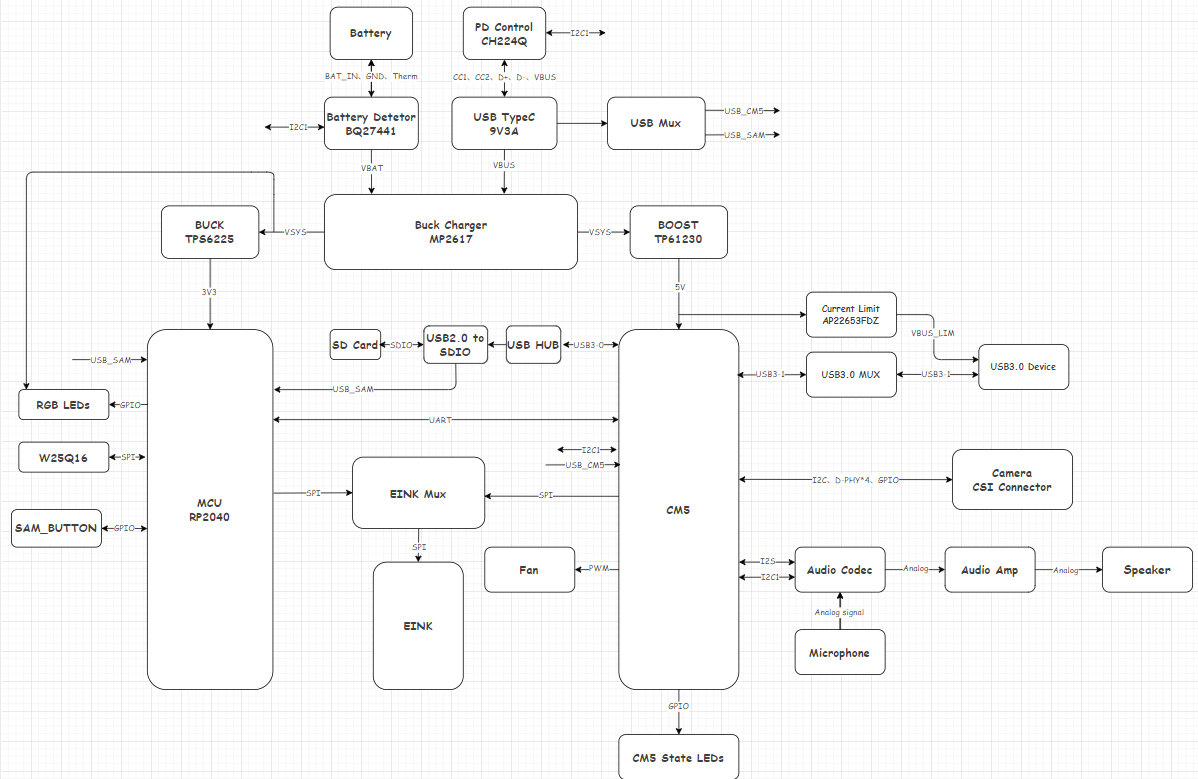
\includegraphics[width=0.8\textwidth]{bhv_hardware_architecture.png}
%     \caption{Distiller BHV Hardware Architecture}
% \end{figure}

\section{SAM Protocol Development}

One of the most significant projects I worked on was the development of the SAM (Signal Aggregation Module) protocol. This was probably my most challenging and rewarding project during the internship.

\vspace{0.3cm}

The Distiller BHV device uses a Raspberry Pi CM5 as the main application processor and an RP2040 microcontroller for handling low-level hardware interfaces. These two components needed to communicate reliably and efficiently.

\vspace{0.3cm}

I designed and implemented the SAM protocol to enable bidirectional communication between the RP2040 and the CM5 over UART. The protocol needed to be simple enough for the resource-constrained RP2040 to implement, yet robust enough to handle various types of data and commands reliably.

\vspace{0.3cm}

The protocol design included defining a message structure, creating a command set for different operations, and implementing error handling mechanisms. I had to think carefully about packet structure, checksums for data integrity, and handling of edge cases.

\vspace{0.3cm}

On the Linux side, I wrote a kernel driver that handles the UART communication, processes incoming packets, and exposes interfaces for userspace applications to interact with the RP2040. The driver needed to be efficient because it would be processing potentially thousands of packets per second.

\vspace{0.3cm}

This project taught me a lot about protocol design, kernel driver development, and the challenges of reliable communication between different processors. It also gave me experience in working at both the firmware level (RP2040) and the kernel level (Linux).

% TODO: Add SAM protocol diagram here
% \begin{figure}[h]
%     \centering
%     \includegraphics[width=0.7\textwidth]{sam_protocol_diagram.png}
%     \caption{SAM Protocol Communication Flow}
% \end{figure}

\section{Distiller SDK Development}

Another major project was the development of the Distiller SDK. The SDK provides userspace APIs that allow application developers to interact with the hardware components of the Distiller devices without having to understand the low-level kernel interfaces.

\vspace{0.3cm}

The SDK needed to support multiple hardware components including audio, camera, e-ink display, and others. I designed the API structure to be intuitive and easy to use while maintaining the flexibility needed for different use cases.

\vspace{0.3cm}

The SDK development involved several components:

\begin{enumerate}[itemsep=0.3cm]
    \item \textbf{Kernel Modules:} I wrote or modified kernel modules to expose the hardware functionality in a way that userspace applications could access.

    \item \textbf{Userspace Libraries:} I created Python libraries that wrapped the kernel interfaces and provided high-level APIs for application developers.

    \item \textbf{Platform Abstraction:} Since the SDK needed to work across multiple hardware platforms (Raspberry Pi CM5, Rockchip RK3568, and RK3576), I had to design abstraction layers that hid platform-specific details from applications.
\end{enumerate}

\vspace{0.3cm}

The SDK initially started as ``distiller-cm5-sdk'' when we were only supporting the Raspberry Pi CM5 platform. However, as the company expanded to support additional platforms, I upgraded it to ``distiller-sdk'' with multi-platform support. This involved significant refactoring to make the code platform-agnostic.

\vspace{0.3cm}

This project taught me about API design, maintaining backward compatibility, and the importance of good abstraction layers in software design.

\section{WiFi Provisioning Service}

All Distiller devices are headless, meaning they don't have a traditional display and keyboard interface. This created a challenge: how do users connect these devices to their wifi networks?

\vspace{0.3cm}

I developed the ``distiller-services'' daemon to solve this problem. This userspace daemon handles wifi provisioning, device management, and other system services.

\vspace{0.3cm}

The wifi provisioning system works by creating a temporary wifi access point that users can connect to with their phones. The device runs a web interface that allows users to select their home wifi network and enter the password. Once configured, the device connects to the user's network and the temporary access point is shut down.

\vspace{0.3cm}

Implementing this required:

\begin{enumerate}[itemsep=0.3cm]
    \item \textbf{Architecture Design:} I designed the overall architecture of the service, determining how different components would interact and ensuring the system would be reliable.

    \item \textbf{Network Management:} I implemented functionality to manage wifi connections, handle network state changes, and ensure reliable connectivity.

    \item \textbf{Web Interface:} I created a simple web interface that users could access from their phones to configure the device.

    \item \textbf{State Persistence:} The service needed to remember network configurations across reboots, so I implemented proper state management.

    \item \textbf{Error Handling:} I had to handle various error scenarios, such as incorrect passwords, network connectivity issues, and unexpected state transitions.
\end{enumerate}

\vspace{0.3cm}

This project taught me about network programming, web development, state management, and the importance of good user experience even in system-level software.

% TODO: Add wifi provisioning flow diagram here
% \begin{figure}[h]
%     \centering
%     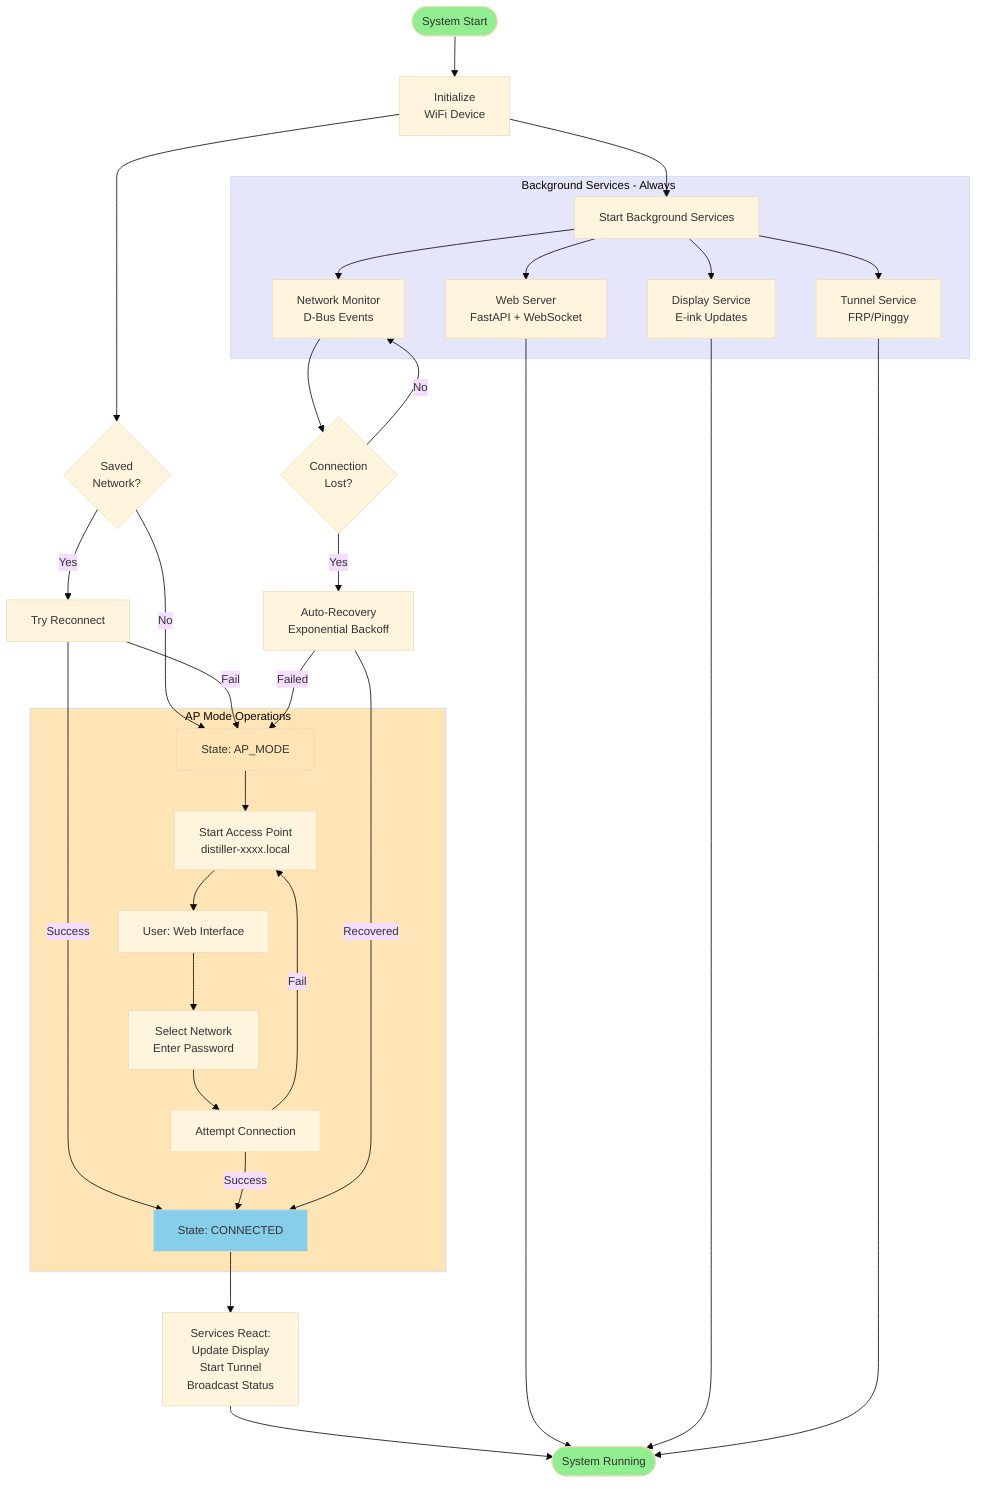
\includegraphics[width=0.8\textwidth]{wifi_provisioning_flow.png}
%     \caption{WiFi Provisioning User Flow}
% \end{figure}

\section{Additional Projects and Contributions}

Beyond the three major projects mentioned above, I contributed to several other initiatives:

\vspace{0.3cm}

\textbf{Distiller CM5 Python Application:} I worked on the complete demonstration application written in Python and QT for the Distiller BHV device. This application ties together all the hardware components (e-ink display, buttons, microphone) to showcase the device's AI capabilities. The application was designed for the DEFCON Bio Hacking Village presentation. Working on this gave me exposure to application-level development and how it integrates with the lower-level systems I had built.

\vspace{0.3cm}

\textbf{APT Server Integration:} I worked on integrating the Distiller device packages with an Aptly-based APT server. This involved creating proper Debian packages for all the software components and setting up the repository structure for easy installation and updates.

\vspace{0.3cm}

\textbf{APT Server CLI:} I developed a command-line interface for managing the APT server. This tool allows the team to easily manage package repositories, handle versioning, and deploy updates.

\vspace{0.3cm}

\textbf{APT Server Portal:} I created a web portal for the APT server that provides a user-friendly interface for managing packages and monitoring device deployments.

\vspace{0.3cm}

\textbf{Regular Tasks:} Throughout the internship, I regularly performed testing of hardware components, debugging issues when they arose, and writing documentation for the drivers and SDKs I developed. These routine tasks were essential for maintaining code quality and ensuring smooth product development.

\section{Technologies and Tools Used}

During the internship, I worked with a diverse set of technologies and tools:

\vspace{0.3cm}

\textbf{Programming Languages:} I primarily used C for kernel driver development, Python for userspace services and applications, and Bash for scripting. I also worked with Rust, JavaScript, TypeScript, HTML, CSS, and QML for various components of the system.

\vspace{0.3cm}

\textbf{Operating Systems:} I worked extensively with Linux, primarily Debian-based distributions. I also used MacOS for some development tasks.

\vspace{0.3cm}

\textbf{Hardware Platforms:} The main platforms I worked with were Raspberry Pi CM5 (using Broadcom BCM2712 SoC), Rockchip RK3568 and RK3576 SoCs, and the RP2040 microcontroller.

\vspace{0.3cm}

\textbf{Development Tools:} I used Neovim as my primary editor, Minicom for serial communication and debugging, Git for version control, Docker for containerization, ClaudeCode for AI-assisted development, and QEMU for some emulation and testing tasks.

\vspace{0.3cm}

\textbf{Build Tools:} I worked with Make for traditional builds and Just (a modern command runner) for more complex build workflows.

\vspace{0.3cm}

The diversity of technologies I worked with gave me broad exposure to different aspects of embedded systems development and helped me understand how different components of a system fit together.

% --------------------------------------------
% CHAPTER 4: LEARNING OUTCOMES AND CHALLENGES
% --------------------------------------------
\chapter{Learning Outcomes and Challenges}

\section{Technical Skills Acquired}

This internship provided me with extensive hands-on experience in several technical areas:

\vspace{0.3cm}

\textbf{Linux Kernel Development:} I gained deep understanding of the Linux kernel architecture, particularly in the areas of device drivers, TTY framework, GPIO framework, and ALSA subsystem. I learned how to write kernel modules, handle kernel APIs, and debug kernel-level issues.

\vspace{0.3cm}

\textbf{Embedded Systems Programming:} Working with multiple SoC platforms taught me about the challenges of embedded systems development, including resource constraints, real-time requirements, and hardware-software integration.

\vspace{0.3cm}

\textbf{Device Driver Development:} I learned how to write drivers for various types of hardware components, from simple GPIO-based devices to complex UART communication interfaces and display drivers.

\vspace{0.3cm}

\textbf{DKMS Modules:} I gained experience in creating DKMS (Dynamic Kernel Module Support) modules, which allow kernel modules to be automatically rebuilt when the kernel is updated. This is essential for maintaining drivers across kernel versions.

\vspace{0.3cm}

\textbf{Debian Packaging:} I learned the complete process of creating Debian packages, including using tools like debuild and lintian to ensure packaging compliance. This knowledge is valuable for deploying software in production environments.

\vspace{0.3cm}

\textbf{Protocol Design:} Designing the SAM protocol taught me how to create robust communication protocols, consider edge cases, and implement error handling mechanisms.

\vspace{0.3cm}

\textbf{System Service Development:} Building the wifi provisioning service gave me experience in developing reliable system-level services that need to handle various states and error conditions gracefully.

\vspace{0.3cm}

\textbf{Multi-Platform Development:} Supporting three different SoC platforms taught me the importance of abstraction layers and platform-agnostic design.

\section{Challenges Faced}

\textbf{E-ink Display Driver:} The e-ink display was one of the hardest challenges I faced. The display had a very unique interface that wasn't covered by any existing Linux driver. I had to carefully study the hardware specifications, understand the timing requirements, and implement the communication protocol from scratch. The difficulty was compounded by the fact that e-ink displays have different refresh characteristics compared to regular displays, and I had to account for these differences in the driver.

\vspace{0.3cm}

\textbf{WiFi Provisioning for Headless Devices:} Designing a user-friendly wifi provisioning system for a headless device was challenging because there's no direct way for users to interact with the device. I had to think creatively about how to make the process as simple as possible while handling all the edge cases that could occur.

\vspace{0.3cm}

\textbf{Introducing Bugs While Adding Features:} Like any development work, I occasionally introduced bugs when adding new features. This taught me the importance of thorough testing, code review, and having good debugging strategies. I learned to write more defensive code and to think through the implications of changes before implementing them.

\vspace{0.3cm}

\textbf{Remote Communication:} Working remotely with a team in a different time zone presented challenges in communication and coordination. I had to be very clear in my written communication and learn to work independently while keeping the team informed of my progress.

\section{Problem-Solving Approaches}

For the \textbf{e-ink display driver}, I approached the problem systematically:

\begin{enumerate}[itemsep=0.2cm]
    \item I started by thoroughly researching the hardware specifications to understand exactly how the display needed to be controlled.
    \item I wrote an initial version of the driver with basic functionality just to test if I could communicate with the display.
    \item I then iteratively improved the driver, testing each addition to ensure it worked correctly.
    \item I consulted with my mentors when I encountered issues I couldn't solve on my own.
\end{enumerate}

\vspace{0.3cm}

For the \textbf{wifi provisioning challenge}, my approach was:

\begin{enumerate}[itemsep=0.2cm]
    \item I designed a service that would create a temporary access point that users could connect to.
    \item I built a simple web interface that could be accessed through a phone's browser.
    \item I conducted extensive testing to handle various scenarios: incorrect passwords, network unavailability, unexpected disconnections, etc.
    \item I implemented proper state management so the system could recover gracefully from errors.
\end{enumerate}

\vspace{0.3cm}

Throughout the internship, I learned that the best approach to solving complex problems is to break them down into smaller, manageable pieces, tackle each piece systematically, and test thoroughly at each step.

\section{Soft Skills Development}

\textbf{Time Management:} Working 6-8 hours per day on multiple projects taught me how to prioritize tasks, manage my time effectively, and meet deadlines. I learned to estimate how long tasks would take and to communicate clearly when I needed more time.

\vspace{0.3cm}

\textbf{Remote Communication:} Working remotely forced me to improve my written communication skills. I learned to write clear, concise messages on Slack, to document my work properly, and to ask questions effectively when I needed help.

\vspace{0.3cm}

\textbf{Independent Problem-Solving:} Since I was working remotely and often on my own, I developed strong independent problem-solving skills. I learned when to persist in solving a problem on my own and when to reach out for help.

\vspace{0.3cm}

\textbf{Adaptability:} Working in a startup environment taught me to be adaptable. Requirements changed, new priorities emerged, and I had to be flexible in adjusting my work accordingly.

\vspace{0.3cm}

\textbf{Collaboration:} Despite working remotely, I learned to collaborate effectively with my team through code reviews, discussions on design decisions, and regular communication about progress and challenges.

% --------------------------------------------
% CHAPTER 5: CONCLUSION
% --------------------------------------------
\chapter{Conclusion}

\section{Overall Experience}

My internship at Pamir AI has been an invaluable learning experience. Working on real-world products in a startup environment gave me exposure to the complete software development lifecycle, from initial design to deployment in production devices.

\vspace{0.3cm}

The opportunity to work directly with the company founders provided me with insights into not just technical development but also product thinking, business strategy, and what it takes to build a successful technology company.

\vspace{0.3cm}

The remote nature of the work, while challenging at times, taught me important skills about self-management, async communication, and working independently. These are skills that will be valuable throughout my career.

\vspace{0.3cm}

Working on multiple aspects of the system, from low-level kernel drivers to high-level application code, gave me a holistic understanding of how complex systems are built and maintained.

\section{Key Achievements}

I am particularly proud of several achievements during this internship:

\begin{enumerate}[itemsep=0.3cm]
    \item \textbf{Complete BSP Development:} I successfully developed complete board support packages for multiple platforms, with proper version control and packaging compliance. This work is now being used in production devices.

    \item \textbf{Production Deployment:} All the work I did, from kernel drivers to system services, is actively being used in Pamir AI's Distiller devices that are in production. Knowing that my code is running on real devices used by real people is very satisfying.

    \item \textbf{Multi-Platform Support:} I successfully implemented support for three different hardware platforms (Raspberry Pi CM5, Rockchip RK3568, and RK3576) from a single codebase, demonstrating good software design and abstraction.

    \item \textbf{Recognition:} My mentors appreciated my dedication and the quality of my work, particularly the custom drivers and the Distiller SDK. This positive feedback validated the effort I put into the work.
\end{enumerate}

\section{Future Implications}

The technical skills I gained in Linux kernel development and embedded systems programming form a strong foundation for my future career in software engineering. These are specialized skills that are in high demand and will open up many career opportunities.

\vspace{0.3cm}

The experience of working in a remote team environment has prepared me well for the modern software industry, where remote and distributed teams are increasingly common.

\vspace{0.3cm}

The exposure to complete product development, including not just coding but also testing, documentation, packaging, and deployment, has given me a comprehensive understanding of what it takes to ship production-quality software.

\vspace{0.3cm}

Most importantly, this internship has confirmed my interest in systems programming and low-level software development. I now have clarity about the direction I want to take in my career and the confidence that I can succeed in this field.

\vspace{0.3cm}

The professional connections I made at Pamir AI and the real-world experience I gained will be valuable assets as I continue my academic journey and eventually transition into full-time employment.

\end{document}
